In this section we describe the design of a virtual machine scheduling system that manages virtual resources and preparation overhead separately, using scheduling strategies designed to increase accuracy and efficiency. In particular, we will discuss (1) how our scheduling system allocates resources for Best-effort and AR requests, (2) a set of file staging strategies for VM image deployment, and (3) a strategy for reusing VM images on physical nodes.

\section{Best-Effort and AR scheduling}
\label{sec:scheduling}

Our system supports scheduling of best--effort requests and closed advance reservation requests (described in Section~\ref{cha:scenarios}). For best--effort requests, we currently only support serial requests, where the individual VMs in a workspace do not need to run in parallel (this is similar to serial batch jobs). Advance reservations, on the other hand, always request VMs in parallel: all the VMs in an advance reservation will begin at the same time, and a request will be rejected if there are not enough resources for all the VMs at the same time.

A best--effort request includes the following information:

\begin{itemize}
\item[---] Number of VMs in the request.
\item[---] Resources required by the VM. We currently support specifying the number of CPUs and amount of memory required by each VM.
\item[---] Maximum duration of each VM.
\item[---] VM image required. This is specified by a URI pointing to the image's location in an image repository node.
\end{itemize}

Best--effort requests are scheduled using a FCFS (First Come First Serve) algorithm. As requests arrive, they are placed on a queue. In turn, the head of the queue is inspected every scheduling quantum, and if there are enough resources to run a single VM at that time, the VM is scheduled for deployment and execution. Since the VMs are serial--scheduled, this process does not involve any backfilling or resource reservation strategies, except in the presence of advance reservations (a case which is explained next).

An advance reservation includes the same information as a best--effort request, but also includes a specific start time at which all the VMs in the request must start. The end time of the reservation will be computed as \emph{start time + duration}. To schedule advance reservations, our scheduler models physical resources as resource slots (as described in the previous section) where we must fit a given request for an advance reservation. To perform this slot--fitting, we first determine if the request it feasible at the requested start and end times and, if there is a choice of physical nodes, we greedily choose the nodes that would minimize the number of image transfers. In particular, we do the following:

\begin{itemize}
\item[---] We have a request for $n$ VMs, starting at time $t_s$ and ending at time $t_e$, each requiring $r_i$ resources (for all $i$ types of resources: CPU, memory, etc.). Each physical node has $R_i$ total resources.
\item[---] Find the physical nodes at time $t$ such that the number of available resources $R_i'$ in each node is $\geqslant r_i$ (i.e., we can fit at least one VM on that node). Make sure that those resources are available up until $t_e$. This is our list of candidate nodes
\item[---] Order the list of candidate nodes, giving priority to nodes where we will be able to reuse already deployed VM images (this is described below in Section~\ref{sec:reuse}), and then to nodes where we can deploy more than one VM. 
\item[---] Traverse the list of candidate nodes and, at each node, fit as many VMs as possible. If we manage to fit all the VMs, we know that the VM component of the reservation is feasible.
\item[---] Before completely accepting the reservation, and committing it in the scheduler, we must check that it will be possible to transfer all necessary VM images by $t_s$. This is described below in Section~\ref{sec:filestaging}
\end{itemize}

\begin{figure}
  \begin{center}
    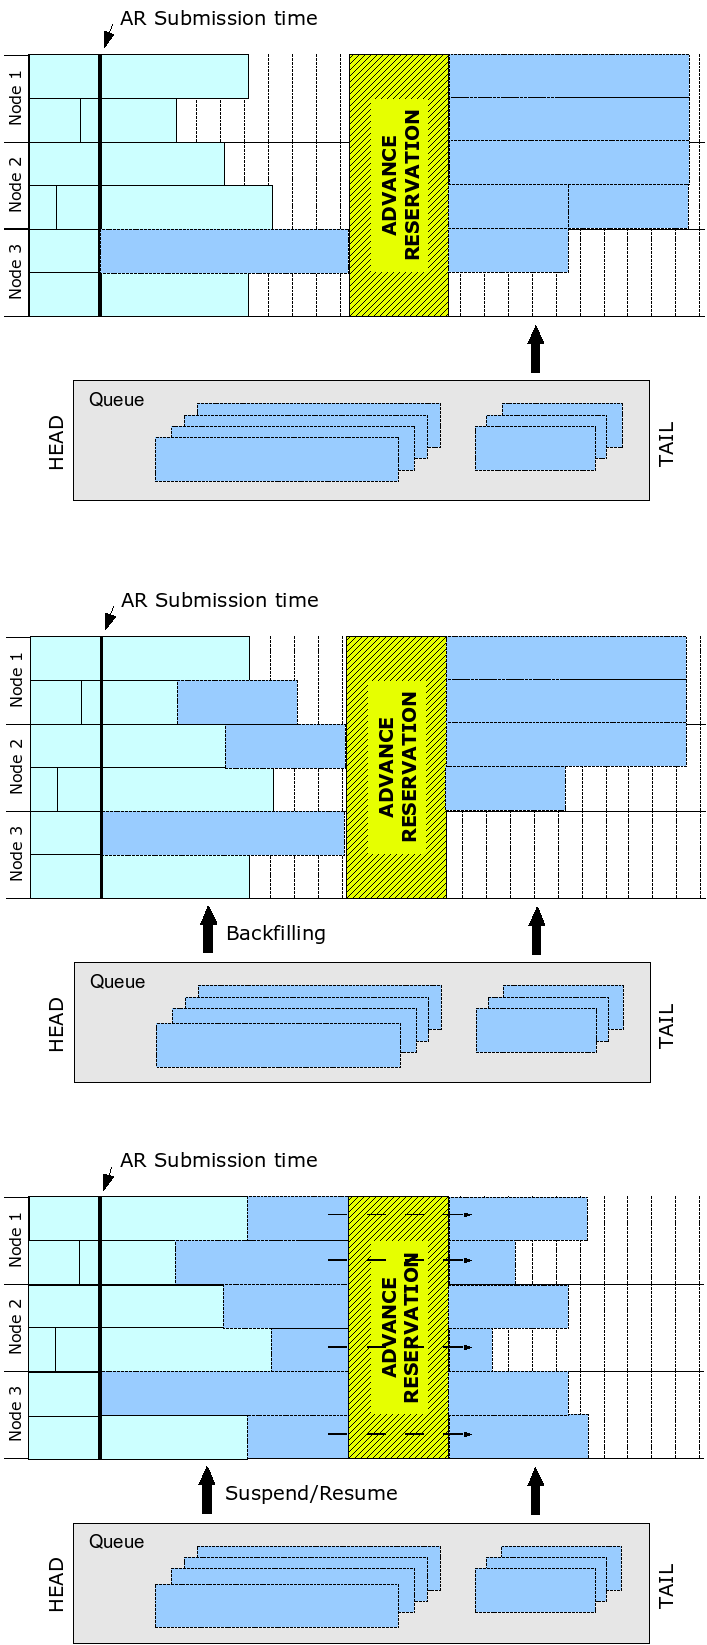
\includegraphics[height=1\textheight]{figures/arbatch.png}
    \caption{Top: Draining nodes before an AR. Middle: Backfilling the time before an AR. Bottom: Suspending before an AR, and resuming after the AR.}
	\label{fig:backfilling}
  \end{center}
\end{figure}


When combining best--effort requests and advance reservations, we can find that the time before an advance reservation is underutilized, as we cannot schedule any best-effort requests that would end after the scheduled start time of the advance reservation (see Figure~\ref{fig:backfilling}, top diagram). This is a common problem in parallel job scheduling, where resources can be allocated for a parallel job (requiring several CPUs in parallel), but the resources before the parallel job might not be able to satisfy the requirements of the next job in the queue. \emph{Backfilling} strategies \cite{10.1109/ICPPW.2002.1039773,feitelson02analyzing,feitelson04parallel} allow lower--priority jobs to run in the time before a parallel job, without affecting the starting times of higher priority jobs (see Figure~\ref{fig:backfilling}, middle diagram).

In a batch scheduler, different backfilling strategies differ on how they reserve resources for parallel jobs in the queue. However, our system does not support parallel best--effort requests (the equivalent of parallel jobs in batch schedulers), and we are only interested in backfilling the time before an advance reservation (which cannot be scheduled on a best--effort basis, like a parallel job) with best-effort serial requests. In this case, the task of backfilling becomes much simpler, and is reduced to traversing the queue in search of VMs which can be scheduled before the advance reservation.

However, as shown in Figure~\ref{fig:backfilling}, backfilling can still result in some underutilization. Another alternative is to suspend best--effort requests before an advance reservation, and resume them as soon as the advance reservation ends (see Figure~\ref{fig:backfilling}, bottom diagram). \emph{Suspend/resume} is not a novel strategy, as many existing resource managers, such as Condor and SGE, allow checkpointing of jobs. However, this feature generally requires modifying a job's executable to support checkpointing, although in some cases this can be achieved by adding checkpointing support to an OS kernel \cite{blcr}. VMs, on the other hand, allow a machine to be suspended/resume seamlessly, without modifying the software that will be running inside the VM.


\section{File staging strategies}
\label{sec:filestaging}

Jobs submitted to batch schedulers generally assume that the required files are available in the worker nodes (e.g., through an NFS drive) or that the input files will be staged to the worker nodes when the job starts. As discussed in the previous section, this assumption presents problems for deploying time{}-sensitive VWs, as VM images can be large and costly to transfer, and transfer times can consume a significant portion of the time allocated to the user. Thus, even if a resource is made available at a requested time $t$, it may not be ready for use until a significantly later time $t+d$.

These problems can be solved in some cases by providing the scheduler with application--specific information about what data needs to be transferred for each deployment, enabling it to distinguish cases where prestaging the data before the scheduled start time $t$ would be appropriate. In the case of a virtual workspace, the application--specific information provided to the scheduler is the workspace metadata file, which contains information the scheduler can use to estimate the amount of preparation overhead (the time necessary to transfer the required VM images). In particular, the relevant information is (1) an image descriptor (currently the location of the image file within an image repository node), (2) the image size, and (3) the number of nodes in the VW.

As described in our virtual resource model, preparation overhead would be managed separately from the virtual resources. Thus, we propose the use of a \emph{scheduled} file transfer strategy: after estimating the amount of preparation overhead, the image transfers are scheduled to complete by time $t$, and the scheduler will reject workspaces where such an image transfer cannot be scheduled (even if all other resources, such as CPU and memory, are available during the requested period of time). In particular, for ARs we schedule image transfers using an Earliest Deadline First (EDF) algorithm \cite{BorjaCite22}. Using EDF allows us to guarantee that image transfers complete by time $t$ (the deadline), while also allowing us to distinguish what image transfers are infeasible. Since EDF is an aggressive algorithm (image transfers begin as soon as possible, even if the deadline is still far away), we also use a just--in--time variation on EDF, which we term EDF/JIT, where image transfer are still sorted according to their deadlines, but pushed as close as possible to the deadline. Figure~\ref{fig:edf} illustrates these two strategies.

\begin{figure}
  \begin{center}
    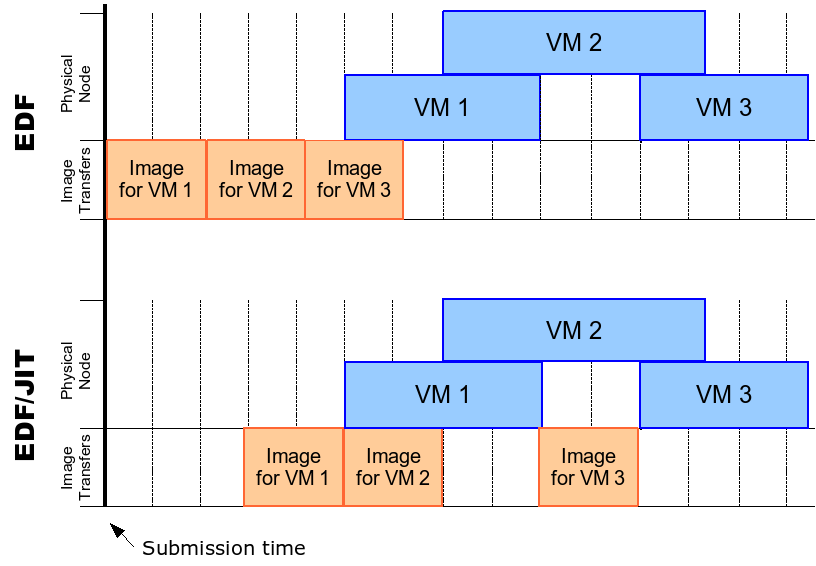
\includegraphics[width=0.8\textwidth]{figures/edf.png}
    \caption{EDF and EDF/JIT file staging strategies}
	\label{fig:edf}
  \end{center}
\end{figure}

Best--effort reservations lack the deadline--sensitive component of AR reservations, so we use a simple FIFO queue to schedule image transfers for these reservations. We currently assume that image transfers for ARs and best--effort reservations are scheduled separately, and we leave the development of an algorithm combining the deadline--sensitive aspect of EDF and the best--effort aspect of FIFO for future work.


\section{Reusing VM images}
\label{sec:reuse}

Adequate VM image staging affects \emph{accuracy}, by making sure that all preparation overhead is processed before the virtual workspace's scheduled start time. We also wish to improve \emph{efficiency} by reducing preparation overhead whenever possible. We accomplish this by reusing VM images already deployed on physical nodes. As described in Section~\ref{sec:vwrepresentation}, factoring deployment--independent configuration information out of the VM image and into a metadata file allows VM images to be reusable. In particular, a VM image can be deployed to a physical machine, and used multiple times by making local copies and binding those copies to potentially different metadata files. This reusability enables us to keep VM image templates on a physical node and using them for several different deployments, thus reducing the number of image transfers.

Our image reuse algorithm requires that each physical node have a certain amount of disk space reserved for an \emph{image pool}. This pool will contain image templates, not bound to any workspace metadata, which can be shared by different deployments. Assuming an empty pool on a node, the deployment of a VW on that node would result in the following steps:

\begin{enumerate}
\item Since the pool is empty, deploying this VW will require transferring an image to that node.
\item Once the transfer is completed, the image is added to the pool, and assigned a \emph{timeout}. This timeout will initially match the end time of the VW, to guarantee that it will remain in the pool for, at least, the duration of the VW.
\item Since we do not want to modify the image (so it can be potentially reused by other VWs), the VW does not use the image in the pool directly. Instead, if the system supports it, it will access the image using \emph{copy--on--write} (COW). If COW is not supported, a local copy of the image will be made before the VW starts.
\item When the timeout of the image is reached, the image is removed from the pool.
\end{enumerate}

Reuse of images is, essentially, accomplished by extending the timeout of the images in the pool to accommodate future deployments. So, let's assume that an image $A$ is deployed, with timeout $t_\textrm{expire}$, on node $N1$, to be used by VW \#1. At some point, a request arrives for VW \#2 starting at time $t_\textrm{start}$ and ending at time $t_\textrm{end}$. If $t_\textrm{start} \leqslant t_\textrm{expire}$ (i.e., the image is guaranteed to be in the image pool at time $t_\textrm{start}$), we flag that image $A$ will also be used by VW \#2, and the timeout will be updated to $t_\textrm{end}$. When $t_\textrm{start}$ arrives, VW \#2 will reuse image $A$ as described above: by using COW or making a local copy.

When scheduling VWs, the scheduler will take into account the state of the image pools in each node, and will attempt to minimize the number of image transfers by allocating, whenever possible, VWs to nodes where the required image is already a part of the image pool. This algorithm also has allows administrators to set a limit on the size of the image pool, making sure that disk usage by VM images will not grow without bounds. The tradeoff, of course, is that some VWs might be rejected since the required VM image is not available in the image pool and cannot be transferred because it would make the image pool too big.

Finally, it should be noted that the strategy of reusing images benefits both AR deployments, since it will be possible to accept starting times that would ordinarily be unfeasible if the image first had to be transferred to the nodes, and best--effort deployments, by allowing workspaces to start running sooner.

\subsection{Avoiding redundant transfers}

\begin{figure}
  \begin{center}
    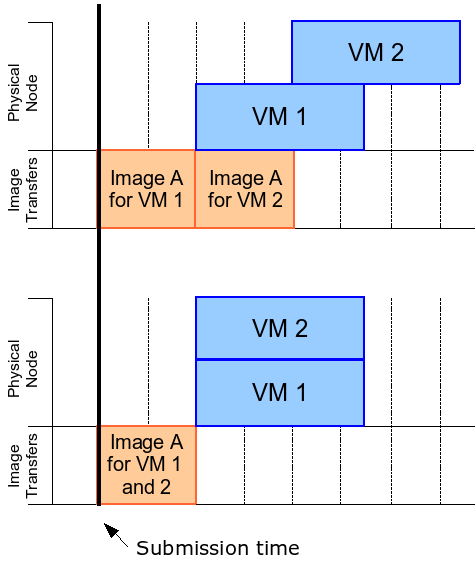
\includegraphics[width=0.6\textwidth]{figures/piggybacking.png}
    \caption{Avoiding redundant transfers}
	\label{fig:piggyback}
  \end{center}
\end{figure}

As an additional optimization to our image reuse algorithm, image transfers are also scheduled in such a way that redundant transfers are avoided. There are two types of redundant transfers we wish to avoid:

\begin{description}
\item[Transfers for ARs:] Assume that a transfer for image $A$ has been scheduled to arrive on node $N1$ at time $t_{1,\textrm{start}}$. This image will be used by VW \#1 (ending at $t_{1,\textrm{end}}$). At some point before $t_\textrm{start}$, a request for VW \#2 arrives, also requiring image $A$, starting at $t_{2,\textrm{start}}$ (where $t_{2,\textrm{start}}>t_{1,\textrm{end}}$) and ending at time $t_{2,\textrm{end}}$. The scheduler determines that VW \#2 should be assigned to node $N1$. Scheduling an additional transfer would be redundant, since there is already a transfer for $A$ scheduled for that node. So, the existing transfer is tagged as carrying an image to be shared by VM \#1 and VM \#2. One the transfer is completed, the image's timeout in the pool will be $t_{2,\textrm{start}}$ (or, more generally, $\textrm{max}(t_{1,\textrm{end}},t_{2,\textrm{end}})$)
\item[Transfers for best--effort reservations:] As shown in Figure~\ref{fig:piggyback} (top), assume that the last image transfer scheduled on the FIFO queue for best--effort reservations carries image $A$ to node $N1$, set to arrive at time $t_\textrm{start}$ to be used by VM \#1. Also, assume that the time to transfer image A is $t_A$. Now, a request for a new best--effort reservation arrives for VM \#2, also requiring image $A$. If we scheduled a separate image transfer for VM \#2, it would start at $t_\textrm{start}+t_A$, despite the availability of resources at $t_\textrm{start}$. By allowing the transfer to piggyback on the previously scheduled transfer, VM \#2 can start earlier, as show in Figure~\ref{fig:piggyback} (bottom)
\end{description}

To avoid these redundant transfers, the scheduler will inspect the image transfer schedule when processing a new request to ascertain if existing image transfers can be reused. In particular:

\begin{description}
\item[Transfers for ARs:] Given a VW starting at time $t_\textrm{start}$ and ending at time $t_\textrm{end}$, requiring image $I$, assigned to node $N$. If there is an image transfer of $I$ scheduled to $N$, with deadline less than or equal to $t_\textrm{start}$, then simply reuse that transfer. Furthermore, the scheduler will take into account existing transfers when mapping requests to nodes (assuming availability of resources in the nodes, it is preferable to schedule a VW to a node with a reusable image transfer than scheduling it to a node where a new image transfer would necessarily have to be scheduled).
\item[Transfers for best--effort:] Given a VW requiring image $I$, the scheduler checks not only the state of the image pools, but also the upcoming transfers in the FIFO transfer queue. This way, it may be possible to schedule a best--effort VW sooner by reusing an existing transfer than by adding an additional transfer to the FIFO queue.
\end{description}





